%%%%%%%%%%%%%%%%%%%%%%%%%%%%%%%%%%%
%This is the LaTeX ARTICLE template for RSC journals
%Copyright The Royal Society of Chemistry 2016
%%%%%%%%%%%%%%%%%%%%%%%%%%%%%%%%%%%

\documentclass[twoside,twocolumn,9pt]{article}
\usepackage{extsizes}
\usepackage[super,sort&compress,comma]{natbib} 
\usepackage[version=3]{mhchem}
\usepackage[left=1.5cm, right=1.5cm, top=1.785cm, bottom=2.0cm]{geometry}
\usepackage{balance}
\usepackage{mathptmx}
\usepackage{sectsty}
\usepackage{graphicx}
\usepackage{amsmath,amssymb}
\let\hbar\relax
\DeclareRobustCommand{\hbar}{{\mathchar'26\mkern-9mu h}}
\usepackage{lastpage}
\usepackage[format=plain,justification=justified,singlelinecheck=false,font={stretch=1.125,small,sf},labelfont=bf,labelsep=space]{caption}
\usepackage{float}
\usepackage{fancyhdr}
\usepackage{fnpos}
\usepackage[english]{babel}
\addto{\captionsenglish}{%
  \renewcommand{\refname}{Notes and references}
}
\usepackage{array}
\usepackage{droidsans}
\usepackage{charter}
\usepackage[T1]{fontenc}
\usepackage[usenames,dvipsnames]{xcolor}
\usepackage{setspace}
\usepackage[compact]{titlesec}
\usepackage{hyperref}
%%%Please don't disable any packages in the preamble, as this may cause the template to display incorrectly.%%%


\usepackage{epstopdf}%This line makes .eps figures into .pdf - please comment out if not required.

\definecolor{cream}{RGB}{222,217,201}

%%%%%%%%% Preamble of the bibliography, can be commented or deleted 
\def\bibpreamble{For the reference section, the style file \texttt{rsc.bst} can be used to generate the correct reference style.\footnotemark[4]
\begin{enumerate}
\item{Citations should appear here in the format A. Name, B. Name and C. Name, \emph{Journal Title}, 2000, \textbf{35}, 3523;} 
\item{A. Name, B. Name and C. Name, \emph{Journal Title, 2000}, \textbf{35}, 3523.}
\end{enumerate}
... \\\\
We encourage the citation of primary research over review articles, where appropriate, in order to give credit to those who first reported a finding. \href{https://www.rsc.org/news-events/articles/2020/jun/rsc-signs-dora/}{Find out more about our commitments to the principles of San Francisco Declaration on Research Assessment (DORA).}}
%%%%%%%%% 

\begin{document}

\pagestyle{fancy}
\thispagestyle{plain}
\fancypagestyle{plain}{
%%%HEADER%%%
\renewcommand{\headrulewidth}{0pt}
}
%%%END OF HEADER%%%

%%%PAGE SETUP - Please do not change any commands within this section%%%
\makeFNbottom
\makeatletter
\renewcommand\LARGE{\@setfontsize\LARGE{15pt}{17}}
\renewcommand\Large{\@setfontsize\Large{12pt}{14}}
\renewcommand\large{\@setfontsize\large{10pt}{12}}
\renewcommand\footnotesize{\@setfontsize\footnotesize{7pt}{10}}
\makeatother

\renewcommand{\thefootnote}{\fnsymbol{footnote}}
\renewcommand\footnoterule{\vspace*{1pt}% 
\color{cream}\hrule width 3.5in height 0.4pt \color{black}\vspace*{5pt}} 
\setcounter{secnumdepth}{5}

\makeatletter 
\renewcommand\@biblabel[1]{#1}            
\renewcommand\@makefntext[1]% 
{\noindent\makebox[0pt][r]{\@thefnmark\,}#1}
\makeatother 
\renewcommand{\figurename}{\small{Fig.}~}
\sectionfont{\sffamily\Large}
\subsectionfont{\normalsize}
\subsubsectionfont{\bf}
\setstretch{1.125} %In particular, please do not alter this line.
\setlength{\skip\footins}{0.8cm}
\setlength{\footnotesep}{0.25cm}
\setlength{\jot}{10pt}
\titlespacing*{\section}{0pt}{4pt}{4pt}
\titlespacing*{\subsection}{0pt}{15pt}{1pt}
%%%END OF PAGE SETUP%%%

%%%FOOTER%%%
\fancyfoot{}
\fancyfoot[LO,RE]{\vspace{-7.1pt}
\includegraphics[height=9pt]{head_foot/LF}}
\fancyfoot[CO]{\vspace{-7.1pt}\hspace{13.2cm}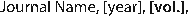
\includegraphics{head_foot/RF}}
\fancyfoot[CE]{\vspace{-7.2pt}\hspace{-14.2cm}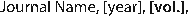
\includegraphics{head_foot/RF}}
\fancyfoot[RO]{\footnotesize{\sffamily{1--\pageref{LastPage} ~\textbar  \hspace{2pt}\thepage}}}
\fancyfoot[LE]{\footnotesize{\sffamily{\thepage~\textbar\hspace{3.45cm} 1--\pageref{LastPage}}}}
\fancyhead{}
\renewcommand{\headrulewidth}{0pt} 
\renewcommand{\footrulewidth}{0pt}
\setlength{\arrayrulewidth}{1pt}
\setlength{\columnsep}{6.5mm}
\setlength\bibsep{1pt}
%%%END OF FOOTER%%%

%%%FIGURE SETUP - please do not change any commands within this section%%%
\makeatletter 
\newlength{\figrulesep} 
\setlength{\figrulesep}{0.5\textfloatsep} 

\newcommand{\topfigrule}{\vspace*{-1pt}% 
\noindent{\color{cream}\rule[-\figrulesep]{\columnwidth}{1.5pt}} }

\newcommand{\botfigrule}{\vspace*{-2pt}% 
\noindent{\color{cream}\rule[\figrulesep]{\columnwidth}{1.5pt}} }

\newcommand{\dblfigrule}{\vspace*{-1pt}% 
\noindent{\color{cream}\rule[-\figrulesep]{\textwidth}{1.5pt}} }

\makeatother
%%%END OF FIGURE SETUP%%%

%%%TITLE, AUTHORS AND ABSTRACT%%%
\twocolumn[
  \begin{@twocolumnfalse}
{
\includegraphics[height=30pt]{head_foot/journal_name}\hfill\raisebox{0pt}[0pt][0pt]{
\includegraphics[height=55pt]{head_foot/RSC_LOGO_CMYK}}\\[1ex]

\includegraphics[width=18.5cm]{head_foot/header_bar}}\par
\vspace{1em}
\sffamily
\begin{tabular}{m{4.5cm} p{13.5cm} }


\includegraphics{head_foot/DOI} & \noindent\LARGE{\textbf{Active-site geometry, not cofactor chemistry, sets the weak-field magnetosensitivity of neurotransmitter-metabolising flavoenzymes$^\dag$}} \\%Article title goes here instead of the text "This is the title"
\vspace{0.3cm} & \vspace{0.3cm} \\

 & \noindent\large{Hikaru Wakaura,$^{\ast}$\textit{$^{a}$} and Taiki Tanimae\textit{$^{a}$}} \\%Author names go here instead of "Full name", etc.

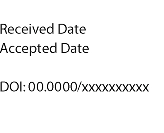
\includegraphics{head_foot/dates} & \noindent\normalsize{That fast recombination and strong exchange coupling suppress weak-field
magnetic effects is established in general terms for the radical-pair mechanism
(RPM). What a general bound cannot say is where a \emph{particular} enzyme falls
--- and it is particular enzymes, the flavoenzymes that metabolise monoamine and
amino-acid neurotransmitters, that recent proposals of geomagnetic influence on
brain chemistry invoke. Using an exact Liouville-space master equation with
spin-selective recombination and electronic dephasing, and radical-pair
parameters fixed by the crystallographic active-site geometry, we compute the
geomagnetic-field ($50\,\mu$T) effect on the singlet yield of monoamine oxidase
A and B and D-amino-acid oxidase. The response is capped by a purely kinetic
ceiling, $(\omega_B\tau)^2 \approx 8\times10^{-7}\,\%$, which follows from the
picosecond active-site lifetime alone and which no coherent mechanism evades;
the computed value is $1.7\times10^{-12}\,\%$, verified to be physical rather
than numerical by its clean $B^2$ scaling over two decades of field. Cryptochrome,
treated in the identical framework, gives $+1.0\,\%$. The discriminating variable
is therefore not the flavin cofactor, which the two share, but the inter-radical
separation that the protein scaffold imposes. We further find the lifetime, not
the exchange coupling, to be decisive: at $\tau\approx10$~ps the response is the
same to within a few per cent whether or not the gigahertz exchange coupling is
present. Neither a quantum-Zeno route nor the $\Delta g$ mechanism restores
sensitivity. The model also says where to test the null: the active-site
singlet--triplet crossing lies at $26.8$~mT, so a fine scan of monoamine-oxidase
turnover through $10$--$40$~mT, not a coarse sweep, is the discriminating
experiment.} \\%The abstrast goes here instead of the text "The abstract should be..."

\end{tabular}

 \end{@twocolumnfalse} \vspace{0.6cm}

  ]
%%%END OF TITLE, AUTHORS AND ABSTRACT%%%

%%%FONT SETUP - please do not change any commands within this section
\renewcommand*\rmdefault{bch}\normalfont\upshape
\rmfamily
\section*{}
\vspace{-1cm}


%%%FOOTNOTES%%%

\footnotetext{\textit{$^{a}$~QIRI (Quantum Integrated Research Institute Inc.), Tokyo 107-0061, Japan. E-mail: h.wakaura@qiri.co.jp}}


%Please use \dag to cite the ESI in the main text of the article.
%If you article does not have ESI please remove the the \dag symbol from the title and the footnotetext below.
\footnotetext{\dag~Electronic supplementary information (ESI) available: solver validation; verification that the reported value is physical rather than a numerical floor ($B^2$ scaling); robustness to hyperfine assignment; quantum Zeno recombination; singlet--triplet dephasing; the $\Delta g$ mechanism; and computational details. See DOI: 00.0000/00000000.}
%additional addresses can be cited as above using the lower-case letters, c, d, e... If all authors are from the same address, no letter is required




%%%END OF FOOTNOTES%%%

%%%MAIN TEXT%%%%
The radical-pair mechanism (RPM) is the only experimentally supported route by
which a magnetic field as weak as the geomagnetic field ($\sim 50\,\mu$T) can
alter the outcome of a chemical reaction~\cite{Steiner1989,Hore2016}. When a
spin-correlated pair of radicals is born in a pure electronic singlet (or
triplet) state, the difference in local hyperfine fields drives coherent
singlet--triplet interconversion; because recombination is spin-selective, an
applied field that re-tunes this interconversion changes the product yields. The
mechanism underlies the leading model of avian magnetoreception, in which the
photoreceptor cryptochrome hosts a flavin--tryptophan radical
pair~\cite{Ritz2000,Maeda2012,Xu2021}.
 
The success of the RPM in cryptochrome has motivated the broader question of
whether other flavoproteins, and in particular the enzymes that metabolise
neurotransmitters, might be magnetosensitive~\cite{Jones2009,ZadehHaghighi2022}.
The question is not purely hypothetical: applied magnetic fields have been
reported to alter monoamine-oxidase activity in brain tissue. Rapidly
alternating fields potentiate MAO-B with an ``active-window'' dependence on the
field slew rate~\cite{Yokoi2000}, and repetitive transcranial magnetic
stimulation inhibits MAO-B in synaptosomal preparations~\cite{Kaczmarczyk2018};
a recent review surveyed the wide range of biological magnetic-field effects
attributed to the RPM and noted its applicability to
neurochemistry~\cite{ZadehHaghighi2022}. These reports involve strong or
time-varying fields. Whether a \emph{weak, static} field such as the geomagnetic
field could bias the catalytic flux of monoamine oxidase (MAO) or D-amino-acid
oxidase (DAO) through the radical-pair mechanism---coupling an environmental
field directly to monoamine and amino-acid neurotransmitter levels---is the
specific, and physiologically consequential, question we address.

This proposal is testable, but a correct test requires three ingredients that
are frequently omitted: a physically realistic radical-pair \emph{lifetime}, the
inter-radical \emph{exchange coupling}, and \emph{electronic decoherence}.
Weak-field sensitivity is fragile. The low-field effect arises from the lifting
of zero-field degeneracies, which opens additional singlet--triplet
pathways~\cite{Lewis2018}, and its magnitude and anisotropy are governed by the
interplay of the hyperfine tensors with the applied field~\cite{Luo2023}; it
therefore demands that coherent singlet--triplet mixing, driven by hyperfine
couplings of order $1$--$10$~mT, survive long enough and remain undamped by
faster competing processes. Treatments that propagate the spin density operator
in the coherent limit, neglect the exchange interaction, and assume a
microsecond lifetime can report sizeable effects that disappear once realistic
kinetics and decoherence are restored.

That this is so \emph{in general} is not in question, and we do not claim it as a
finding. Binhi has recently reviewed the field and, from an analytic treatment of
a two-electron--one-nucleus pair, established in general terms both that primary
chemical RPM effects in biochemistry are of order $10^{-3}$--$10^{-4}$ or
smaller, and that the widely assumed radical-electron decoherence times in
proteins exceeding $1\,\mu$s are not substantiated~\cite{Binhi2025}. We take that
result as our starting point rather than our conclusion. A general
relaxation-limited bound is regime-general by construction: it applies with equal
force to cryptochrome, which \emph{is} a functional magnetoreceptor, and to
monoamine oxidase, which has been claimed to be one. It cannot by itself
adjudicate between them, and it returns no number for any named enzyme. Three
things are therefore still missing, and a neurochemical claim needs all three:
how far below the general bound a given active site actually falls once its
parameters are fixed by its own crystal structure; which physical
factor---lifetime, exchange coupling, or decoherence---does the suppressing,
since only the decisive factor can be argued about experimentally; and what
measurement would overturn the verdict.

Here we supply those three for the neurotransmitter-metabolising flavoenzymes. We
compute the magnetic field effect (MFE) on the singlet yield of MAO-A, MAO-B, DAO,
and---as a positive control in the identical framework---cryptochrome, using an
exact Liouville-space master equation that includes spin-selective recombination
and electronic dephasing. Three results follow. First, a quantitative
enzyme-specific bound: the active-site pairs respond at $1.7\times10^{-12}\,\%$,
capped robustly by a purely kinetic ceiling $(\omega_B\tau)^2\approx
8\times10^{-7}\,\%$ that the picosecond lifetime imposes on its own; cryptochrome,
same code and same numerics, returns $+1.0\,\%$. Second, an attribution: it is
the lifetime, not the gigahertz exchange coupling, that is decisive at
$\tau\approx10$~ps---which relocates the argument from a quantity nobody can
measure in this system to one that can be. Third, a falsifiable consequence: the
singlet--triplet crossing of the active-site pair lies at $26.8$~mT, so the
discriminating experiment is a fine field scan through the tens-of-millitesla
range. The contribution is not that weak-field effects are small---that is
known---but that magnetosensitivity is decided by the geometry the protein
scaffold imposes on the pair rather than by the cofactor it carries, and by how
much.

\section{Methods}

\subsection{Spin Hamiltonian}

Each enzyme is modelled as a two-electron radical pair coupled to the dominant
hyperfine nuclei. For the flavin-centred radical these are the isoalloxazine
ring nitrogens and protons, with isotropic couplings of order $10$--$20$~MHz;
the partner radical is identified per enzyme in Table~\ref{tab:params}. The spin
Hamiltonian (in angular-frequency units, $\hbar = 1$) is
\begin{align}
H &= \omega_B\,(S_{1z}+S_{2z})
   + \sum_{i} \mathbf{S}_1\!\cdot\! \mathsf{A}_i \!\cdot\! \mathbf{I}_i
   \nonumber\\
  &\quad
   + J\,\mathbf{S}_1\!\cdot\!\mathbf{S}_2
   + \mathbf{S}_1\!\cdot\! \mathsf{D}\!\cdot\! \mathbf{S}_2 ,
\label{eq:H}
\end{align}
where $\omega_B = g\mu_B B/\hbar$ is the electron Zeeman frequency at field $B$
($g\approx2$), $\mathbf{S}_{1,2}$ are the two electron spins, $\mathsf{A}_i$ are
the isotropic hyperfine tensors coupling electron~1 to the dominant ring nuclei
$\mathbf{I}_i$, $J$ is the isotropic inter-radical exchange coupling, and
$\mathsf{D}$ is the electron--electron dipolar tensor. We retain the dominant
isotropic hyperfine terms and treat the dipolar coupling in the point-dipole
approximation at the inter-radical distance $r$. The computational model carries
five spins: the two electrons plus three dominant hyperfine-coupled nuclei (two
on the flavin radical, one on the partner), giving a $32$-dimensional Hilbert
space. The conclusions are insensitive to the precise hyperfine assignment,
which controls only the field scale at which a \emph{separated} pair would
respond, not the verdict for the active-site pairs (ESI,\dag~Table~S2).

\subsection{Master equation}

The radical pair is born in the singlet state, $\rho_0 = P_S/\mathrm{Tr}\,P_S$,
where $P_S = \tfrac14 - \mathbf{S}_1\!\cdot\!\mathbf{S}_2$ projects onto the
electronic singlet and $P_T = I - P_S$ onto the triplet manifold. Its
density operator evolves under
\begin{equation}
\frac{d\rho}{dt} = -i[H,\rho]
  - \tfrac12\{k_S P_S + k_T P_T,\,\rho\}
  + \sum_{i=1,2}\frac{1}{T_2^e}\!\left(S_{iz}\,\rho\,S_{iz} - \tfrac14\rho\right).
\label{eq:me}
\end{equation}
The second term is the Haberkorn spin-selective recombination
superoperator~\cite{Haberkorn1976}, with singlet and triplet recombination rates
$k_S$ and $k_T$. The final term is electronic pure dephasing of each electron
spin at rate $1/T_2^e$, which damps the singlet--triplet coherence that the
hyperfine interaction generates. We take $k_S = k_T = k = 1/\tau$ so that the
recombination lifetime $\tau$ enters as a single rate; making recombination
strongly singlet-selective does not enhance the weak-field effect.

The observable is the time-integrated singlet yield,
$\Phi_S = k_S \int_0^{\infty}\!\mathrm{Tr}[P_S\,\rho(t)]\,dt$. This steady-state
expression is a standard consequence of Eq.~\eqref{eq:me}: writing the
Liouvillian $\mathcal{L}$ for the right-hand side and vectorising the density
operator, the integral is performed in closed form,
\begin{equation}
\Phi_S = k_S\, \mathrm{vec}(P_S)^{\dagger}\,(-\mathcal{L})^{-1}\,\mathrm{vec}(\rho_0),
\label{eq:yield}
\end{equation}
which we evaluate by exact linear solution in the $32^2$-dimensional Liouville
space; in the coherent, symmetric-recombination limit this reproduces the
closed-form Green's-function singlet yield to machine precision (electronic
supplementary material, S1). The magnetic field effect is
$\mathrm{MFE}(B) = [\Phi_S(B) - \Phi_S(0)]/\Phi_S(0)$, reported at
$B = 50\,\mu$T. All four enzymes were propagated with identical numerics; only
the per-enzyme parameters differ.

\subsection{Parameters}

The per-enzyme exchange coupling, lifetime, and electronic coherence time are
collected in Table~\ref{tab:params}. The exchange coupling follows the standard
exponential distance dependence $J(r) = J_0\,e^{-\beta r}$ with
$\beta\approx1.4$~\AA$^{-1}$, the standard decay constant for through-protein
electron exchange~\cite{Efimova2008,Moser1992}; this is an order-of-magnitude
estimate, but the
conclusions depend only on whether $|J|$ is large or small compared with the
hyperfine scale ($\sim$tens of MHz), not on its precise value. At the
active-site inter-radical distance of the flavoenzymes ($r\approx3.5$--$4$~\AA),
this gives $|J|\sim0.4$--$0.75$~GHz; for the spatially separated cryptochrome
pair ($r = 15$--$20$~\AA), $|J| < 1$~MHz, effectively zero. That the
inter-radical exchange and dipolar couplings quench the weak-field response
unless the radicals are separated by more than $\sim$$3.5$~nm is an established
result of radical-pair compass theory~\cite{Efimova2008}; the present
calculation applies it to the active-site geometry of the metabolic enzymes. For
the separated cryptochrome pair, spin relaxation analyses place the relevant
electronic coherence in the microsecond range~\cite{Kattnig2016}, consistent
with the coherence-favourable value adopted here.

Lifetimes are fixed by the chemistry. In the flavoenzyme active site the radical
pair, if it forms at all, recombines by ultrafast back electron transfer. At the
van der Waals donor--acceptor contact of the active site ($r\approx3.5$~\AA),
empirical electron-transfer rate laws place the transfer rate at
$\sim10^{11}$--$10^{12}$~s$^{-1}$, i.e.\ $\tau\sim1$--$10$~ps~\cite{Moser1992}; we
adopt the conservative (long) end, $\tau\sim10$~ps ($k\sim10^{5}$~MHz). The
stopped-flow flavin-reduction kinetics measured for
MAO~\cite{Ramsay1991,Vianello2012,Edmondson2004main} bound the overall catalytic
turnover, not this putative intermediate, and are orders of magnitude slower. The
precise value is not critical: Fig.~\ref{fig:honest}a shows the active-site effect
stays below $4\times10^{-6}\,\%$ even for a lifetime $10^{5}$ times longer, because
the gigahertz exchange coupling---not the lifetime---sets the ceiling. In
cryptochrome the
electron-transfer chain spatially separates the radicals and the pair survives
into the microsecond regime ($k\sim1$~MHz,
$\tau\sim1\,\mu$s)~\cite{Maeda2012,Hiscock2016}. The two regimes also have
physically distinct coherence environments. At the active site the radicals
share a small, rigid pocket, where the gigahertz exchange and dipolar couplings,
a dense local hyperfine bath, and picosecond recombination together hold the
electronic coherence to the nanosecond range, $T_2^e\sim1$~ns. In the spatially
separated cryptochrome pair the radicals are mutually isolated and weakly
coupled, and spin-relaxation analyses place the electronic coherence in the
microsecond range~\cite{Kattnig2016}; we adopt a coherence-favourable $T_2^e$ up
to the lifetime as the most optimistic case. These are different physical
environments, not a single dephasing mechanism scaled by three orders of
magnitude. The disparity is moreover not load-bearing for the null result: the
active-site effects are already $\sim\!1.7\times10^{-12}\,\%$ in the coherent limit
($T_2^e\to\infty$, Table~\ref{tab:params}), so the bound holds for \emph{any}
active-site coherence time; for this regime decoherence only tightens it. The electronic-structure inputs---hyperfine
magnitudes and inter-radical distances---were taken from semi-empirical GFN2-xTB
calculations on the relevant crystal structures~\cite{Bannwarth2019}
cross-checked against published ENDOR hyperfine couplings for flavin
radicals~\cite{Weber1998}; the MAO active-site geometry is that resolved
crystallographically~\cite{Edmondson2004main}.

\section{Results}

\subsection{The null result}

Table~\ref{tab:params} reports the calculated MFE at $50\,\mu$T for all four
enzymes. For MAO-A, MAO-B, and DAO the geomagnetic-field effect on the singlet
yield is of order $10^{-12}\,\%$ at the physical picosecond lifetime, both in the
coherent limit and with realistic electronic decoherence. Even in the most
favourable case for an active-site pair---the coherent limit with an unphysically
long lifetime---the exchange and dipolar couplings together cap the effect at
$4.0\times10^{-6}\,\%$ (Fig.~\ref{fig:honest}a). We stress that these are
model-internal values for the five-spin Hamiltonian of Eq.~(1): they quantify the
response of the model, not a rigorous bound on the enzyme. They are, however,
physical values and not an artefact of finite-precision arithmetic: the computed
MFE follows the perturbative $B^2$ law to better than $0.3\,\%$ from $100\,\mu$T
to $25$~mT, and extrapolating that converged slope back to $50\,\mu$T reproduces
the tabulated numbers to within $1.4\,\%$ (ESI,\dag~Table~S1). A numerical floor
would exhibit no such scaling. Because the effect
already vanishes in the coherent limit, the active-site null is independent of
the assumed electronic coherence time: the value of $T_2^e$ cannot be the origin
of the contrast with cryptochrome, which follows instead from the exchange
coupling and lifetime alone. Cryptochrome, by
contrast, shows a clear effect of $+1.0\%$ with decoherence included ($+2.0\%$ in
the coherent limit), of the sign and order of magnitude expected for a functional
magnetoreceptor. This is an optimistic-coherence estimate---we assign
cryptochrome an electronic coherence time up to its lifetime---so the true value
lies below it; measured in-vitro flavoprotein field effects at weak field are
typically at or below the one-percent level~\cite{Maeda2012,Hore2016}. The robust
point is the contrast: the neurotransmitter-metabolising flavoenzymes are
magnetically inert at the geomagnetic field by some twelve orders of magnitude
relative to cryptochrome.

This bound is consistent with what experiment reports. The one study to scan
\emph{static} field strengths on brain monoamine oxidase found no change in
either MAO-A or MAO-B activity from $0.1$ to $340$~mT~\cite{Yokoi2000}; the
potentiation reported in that work appeared only for rapidly alternating fields,
which drive the enzyme through a non-equilibrium, time-dependent mechanism
distinct from the weak-static-field RPM analysed here. Our calculation supplies
the mechanistic reason for that static-field null and extends it down to the
geomagnetic range.

\subsection{Why the active-site pairs are inert}

Figure~\ref{fig:honest} explains the null result physically. Panel~(a) plots the
geomagnetic-field $|\mathrm{MFE}|$ against the radical-pair lifetime $\tau$ for
two geometries: a spatially separated pair with $J\approx0$, and an active-site
pair with $J = 750$~MHz. For the separated pair (blue), the effect grows with
lifetime and only becomes appreciable once $\tau$ exceeds roughly $100$~ns,
because singlet--triplet interconversion driven by sub-millitesla hyperfine
fields needs hundreds of nanoseconds to develop. The flavoenzyme regime
($\tau\approx10$~ps, shaded) sits far to the left, where the effect falls below
$\sim\!1.7\times10^{-12}\,\%$ for \emph{both} geometries---at this lifetime the
exchange coupling barely matters: picosecond recombination freezes the spin state before any
singlet--triplet mixing can occur. Independently, the active-site pair (red),
even if given a long lifetime, saturates at $|\mathrm{MFE}|\sim 4.0\times10^{-6}\,\%$
because its large exchange coupling holds the singlet and triplet levels far
apart in energy, so a $50\,\mu$T field cannot bring them into resonance. Either
mechanism---the picosecond lifetime or the gigahertz exchange coupling---suffices
to suppress the effect; the flavoenzymes have both.

Panel~(b) shows that for the separated geometry electronic decoherence tightens the bound. For the most
favourable separated-pair case ($\tau = 1\,\mu$s, $J\approx0$), $|\mathrm{MFE}|$
collapses as the electronic coherence time $T_2^e$ falls below $\sim100$~ns;
recovering a weak-field effect requires \emph{both} $\tau\gtrsim100$~ns
\emph{and} $T_2^e\gtrsim100$~ns. The active-site value $T_2^e\sim1$~ns lies two
orders of magnitude below this threshold.

\subsection{Why coherent-limit treatments overestimate the effect}

If the dephasing term of Eq.~\eqref{eq:me} is dropped \emph{and} a microsecond
lifetime is assigned to the active-site pair, the same model returns percent-level
MFEs for the flavoenzymes. Both assumptions are required: the long lifetime lets
singlet--triplet mixing run to completion, and omitting decoherence prevents that
mixing from dephasing. Neither holds for an active-site radical pair, where back
electron transfer is picosecond-fast and hyperfine-induced dephasing is
nanosecond-fast. A coherent-limit treatment that makes these two assumptions for
an active-site pair will therefore overestimate the weak-field effect by orders
of magnitude. We do not claim that any particular earlier study is in error---a
given treatment may have addressed a different geometry, mechanism, or parameter
regime---but rather state the methodological boundary: an RPM estimate for an
active-site cofactor radical must propagate the physical lifetime and electronic
decoherence, or it will overstate the effect by orders of magnitude.

\subsection{Mechanistic caveat}

A further point strengthens, rather than weakens, the negative conclusion. It is
not established that MAO catalysis proceeds through a discrete radical-pair
intermediate at all. Multireference CASSCF(2,2)/NEVPT2 calculations on a
lumiflavin--methylamine model~\cite{Sun2020,Angeli2001,Nakano2017} give only weak
diradical character along the hydrogen-transfer coordinate
(Fig.~\ref{fig:casscf}): the diradical index is $y_0 = 0.03$--$0.09$ and the
singlet--triplet gap is $3.2$--$4.1$~eV across the relevant
$d(\mathrm{N5}\cdots\mathrm{H})$ range. Such values favour a polar or concerted
hydride/proton-coupled pathway over genuine radical-pair
formation~\cite{Vianello2012}, in agreement with QM/MM studies of MAO catalysis
that find no radical intermediate and support a concerted asynchronous polar
nucleophilic mechanism~\cite{Repic2013}. This calculation is deliberately
suggestive rather than definitive: it samples three geometries with a minimal
CAS(2,2) active space on a reduced lumiflavin--methylamine model, and does not by
itself exclude a radical-pair intermediate in the full enzyme. We present it only
as an independent, consistent indication; the central result of the paper---the
weak-field bound---does not depend on it, since that bound holds \emph{whether or
not} an active-site radical pair forms. If one does not, the RPM does not apply;
if one does, its geomagnetic effect is the negligible value computed above.

\section{Discussion}

The picture that emerges is that magnetosensitivity is not a generic property of
flavoprotein cofactor radicals; it must be engineered. Cryptochrome achieves it
with a purpose-built electron-transfer chain---the tryptophan triad---that
separates the two radicals by $15$--$20$~\AA, quenching the exchange coupling and
extending the lifetime into the microsecond regime where a $50\,\mu$T field can
act~\cite{Ritz2000,Maeda2012,Xu2021,Hiscock2016}. The
neurotransmitter-metabolising flavoenzymes have the opposite geometry: their
chemistry happens in a tight active site, where any radical pair recombines in
picoseconds and feels a gigahertz exchange splitting. Each factor alone forbids a
weak-field effect; together they place it near $10^{-12}\,\%$, with realistic
electronic decoherence pushing it lower still. The geomagnetic field cannot
meaningfully bias the singlet yield of an active-site radical pair in MAO-A,
MAO-B, or DAO, and proposals that it modulates monoamine or amino-acid
neurotransmitter levels through the RPM are not supported.

\subsection{Relation to the general relaxation-limited bound}

That fast recombination and strong exchange coupling suppress weak-field effects
is established, and Binhi's recent review gives it in closed form for a
two-electron--one-nucleus pair, together with a catalogue of protein relaxation
channels that places generic biological RPM effects at $10^{-3}$--$10^{-4}$ or
below and rejects the routine assumption of microsecond electron decoherence in
proteins~\cite{Binhi2025}. Our results are consistent with that analysis, and
where they overlap they corroborate it from an independent direction: the
nanosecond $T_2^e$ assigned here to a shared, rigid active-site pocket is reached
from the active-site geometry rather than from a relaxation-mechanism catalogue.
Three things nevertheless separate the present calculation from the general
result, and a claim about neurochemistry needs all three.

First, a regime-general bound cannot discriminate. Whatever forbids weak-field
sensitivity in monoamine oxidase must be reconciled with cryptochrome, where
weak-field sensitivity is observed~\cite{Maeda2012}. The present calculation
returns $1.7\times10^{-12}\,\%$ and $+1.0\,\%$ for the two \emph{in the same code
with the same numerics and the same five-spin model}; what separates them is the
inter-radical separation the protein scaffold imposes, not the flavin cofactor
they share. That contrast, rather than the smallness of either number, is the
result of this paper.

Second, these enzymes fall far below the general estimate, by an amount only
enzyme-specific parameters can supply. The generic $10^{-3}$--$10^{-4}$ figure is
a \emph{relaxation}-limited bound. What actually binds at a flavoenzyme active
site is \emph{kinetic}: $(\omega_B\tau)^2 \approx 7.8\times10^{-7}\,\%$, fixed by
the picosecond lifetime that the crystallographic van der Waals donor--acceptor
contact enforces through the Moser--Dutton rate law~\cite{Moser1992}. This
ceiling is some four orders of magnitude tighter than the generic figure, is
independent of every relaxation parameter, and the computed response lies a
further five orders below it. Neither number is available from a general
analysis, because neither survives without the crystal structure.

Third, a general bound identifies no experiment. Because the suppression here is
lifetime-dominated rather than exchange-dominated---a distinction the general
treatment does not draw---the falsifying observation is specific and is stated
below: a resonant feature at the $26.8$~mT singlet--triplet crossing would show
that the active-site pair lives orders of magnitude longer than assumed.

Two limitations of scope should be stated plainly. First, the computed observable
is the time-integrated singlet yield of an isolated pair, not a turnover number.
We take $k_S = k_T$, for which the total recombination flux is field-independent
by construction; the bound is therefore on the spin-selective branching that any
RPM-based effect on catalysis would have to exploit, not on the enzymatic rate
itself. Since $\Phi_S$ is the quantity any downstream spin-selective step must
read, bounding it does bound the achievable RPM effect---but connecting the two
quantitatively would require a kinetic scheme with distinct singlet and triplet
product channels, which we have not constructed. Second, we have not simulated
radical-triad or scavenger mechanisms, in which a third radical restores
magnetosensitivity to a pair that is insensitive on its own~\cite{Kattnig2017}.
Such schemes require the pair to survive long enough to encounter the third
spin, which is implausible on a $10$~ps timescale, but we have not tested this
and it remains the most plausible route by which our conclusion could fail for a
longer-lived intermediate.

One recent result deserves explicit attention. It has been shown that a tightly
bound radical pair---one with a large exchange coupling, of the kind found at an
enzyme active site---can nonetheless become sensitive to an Earth-strength field
when its recombination is strongly spin-asymmetric, through a quantum Zeno
mechanism~\cite{Denton2024}. This appears to contradict the present conclusion,
so we tested it directly: for the monoamine-oxidase parameters
($|J| = 750$~MHz, $\tau\approx10$~ps) we recomputed the MFE with strongly
asymmetric recombination, varying $k_S/k_T$ over six orders of magnitude. The
geomagnetic-field MFE remained below $10^{-7}\,\%$ for every asymmetry, and even at a
$200$-fold stronger field ($10$~mT) it did not exceed $1.5\times10^{-3}\,\%$
(ESI,\dag~Table~S3). The
quantum Zeno mechanism cannot rescue magnetosensitivity here because it requires
the recombination to act over a window in which spin evolution can be projected;
the picosecond active-site lifetime is too short for any such window to open. The
Zeno route to weak-field sensitivity in tightly bound pairs therefore applies to
longer-lived species (for example a flavin--superoxide pair~\cite{Denton2024,Player2019})
but not to the picosecond active-site radical pair of a metabolic flavoenzyme.

The null is likewise insensitive to the form of the electronic decoherence. For a
tightly bound pair the dominant channel is expected to be singlet--triplet
dephasing driven by fluctuations in the exchange coupling, whose Lindblad
operator ($\propto P_S - P_T$) differs from the single-spin channel used above.
Adding this channel at any rate up to and beyond the exchange coupling leaves the
geomagnetic-field MFE far below the level of interest (ESI,\dag~Table~S4). We emphasise that this is an empirical result for the two channels
examined, not a general theorem: because the MFE is a \emph{ratio}, a dissipative
channel acts on $\Phi_S$ at zero and at finite field alike and can in principle
\emph{increase} it. Our own model provides an example---for a long-lived
($\tau = 1\,\mu$s) pair at $J = 750$~MHz, introducing $T_2^e = 1$~ns changes the
geomagnetic-field MFE from $-1.4\times10^{-6}\,\%$ to $+3.6\times10^{-4}\,\%$, a
change of sign and two orders of magnitude. The picosecond active-site regime
studied here is not subject to this, but the choice of dephasing model must be
justified rather than assumed to be conservative.

We also tested the $\Delta g$ mechanism, the one coherent channel that survives
when the exchange coupling greatly exceeds the hyperfine scale and therefore the
natural candidate for rescuing a strongly coupled pair. At the realistic value
$\Delta g \simeq 10^{-3}$ the geomagnetic-field MFE is unchanged, and even at
$\Delta g = 3\times10^{-2}$ it reaches only $3\times10^{-10}\,\%$ (ESI,\dag~Table~S5). The underlying reason is a scale hierarchy that no
coherent mechanism evades: the recombination rate $1/\tau = 10^{5}$~MHz exceeds
the largest internal coupling ($|D| = 1214$~MHz) by more than two orders of
magnitude, and the field enters only through $\omega_B$, so the response is
bounded by $(\omega_B\tau)^2 \approx 7.8\times10^{-9}$---that is,
$7.8\times10^{-7}\,\%$---however the remaining couplings are arranged. This
ceiling lies some five orders of magnitude above the computed response and still
about five orders below the $\sim\!0.1\,\%$ level at which in-vitro magnetic
field effects are detectable. This is why the active-site and separated geometries
agree to within a few per cent at $\tau = 10$~ps despite differing by three
orders of magnitude in $J$.

This bound concerns the RPM specifically. It does not exclude all conceivable
magnetic influences on neurochemistry---for example field effects mediated by
reactive-oxygen-species partitioning~\cite{Usselman2016,Player2019} or other
non-radical-pair channels---but those would require their own mechanism and
evidence and are not addressed by a singlet-yield calculation. A separate and
unrelated proposal, Fisher's suggestion that Posner molecules store quantum
information in $^{31}$P nuclear spins~\cite{Fisher2015}, invokes nuclear rather
than electronic spin coherence; it is a different mechanism, equally unconfirmed,
and our electronic-spin bound says nothing for or against it.

The conclusion is experimentally falsifiable, and the model identifies where to
look. The electron Zeeman splitting matches the active-site exchange coupling
($J = 750$~MHz) at $B = 26.8$~mT, so the singlet--triplet level crossing of the
active-site pair lies not at Tesla fields but inside the tens-of-millitesla
range. In our model a \emph{long-lived} pair with this exchange coupling shows a
large resonant response there (tens of per cent at $\tau = 1\,\mu$s), while the
physical picosecond pair shows $\sim\!5\times10^{-7}\,\%$. The discriminating
experiment is therefore not a coarse $0$--$50$~mT sweep but a fine scan through
the crossing: measuring steady-state MAO turnover from $10$ to $40$~mT in
$\sim\!1$~mT steps should return a null result. A resonant feature near $27$~mT
would not require physics beyond the standard RPM---it would indicate that the
active-site radical pair lives orders of magnitude longer than assumed here,
which is the single assumption on which our conclusion rests.

\subsection{Relation to a previous preprint by the authors}

An earlier version of this work was deposited by the authors on Research Square
and has not been peer reviewed~\cite{Wakaura2026preprint}. The present manuscript
differs from it in substance, not only in presentation. (i) \emph{The observable
has changed.} The preprint reported a bound on ``catalytic flux'', a quantity a
singlet-yield calculation does not deliver; here the computed observable is the
time-integrated singlet yield and the limits of that scope are stated explicitly.
(ii) \emph{The mechanistic attribution has changed}, which is why the title has
changed. The preprint attributed the suppression to electronic decoherence and
exchange coupling; the present calculation identifies the picosecond lifetime as
decisive---at $\tau\approx10$~ps the response is unchanged to within a few per
cent when the gigahertz exchange coupling is removed, and the null already holds
in the coherent limit, so decoherence cannot be its origin. (iii) \emph{The bound
is now quantitative and verified.} The preprint quoted $<10^{-4}\,\%$; here we
give $1.7\times10^{-12}\,\%$, the analytic ceiling $(\omega_B\tau)^2$, and a
$B^2$-scaling test establishing that the value is physical rather than numerical
(ESI,\dag~Table~S1). (iv) \emph{Four robustness analyses have been added} that
the preprint did not contain: the quantum Zeno mechanism~\cite{Denton2024},
singlet--triplet dephasing, the $\Delta g$ mechanism, and a multireference
CASSCF(2,2)/NEVPT2 test of whether a radical pair forms at all. (v) \emph{An
over-strong claim has been withdrawn.} The preprint asserted that percent-level
results in the prior literature are ``computational artifacts''; that assertion
is replaced here by a statement of the methodological requirement, since we
cannot audit parameter choices made for a different geometry or mechanism.

\section{Conclusions}

That fast recombination and strong exchange coupling suppress weak-field
magnetosensitivity is known in general terms~\cite{Binhi2025}. What has been
missing is where named enzymes fall, which factor puts them there, and what would
show otherwise. Using an exact Liouville-space master equation with electronic
decoherence and radical-pair parameters fixed by crystallographic active-site
geometry, we find the geomagnetic-field effect on the singlet yield of the
putative active-site radical pairs of MAO-A, MAO-B and DAO to be
$1.7\times10^{-12}\,\%$, capped robustly at $(\omega_B\tau)^2\approx
7.8\times10^{-7}\,\%$ by the picosecond lifetime alone---four orders of magnitude
below the generic relaxation-limited estimate for a biological radical pair, and
reached without reference to any relaxation parameter. Cryptochrome, in the same
model, returns $+1.0\,\%$. The decisive variable is therefore the inter-radical
separation the protein scaffold imposes and not the flavin cofactor the two
enzymes share: magnetosensitivity in a flavoprotein is a property of geometry,
which must be built, rather than of cofactor chemistry, which comes for free.
Within the active site the suppression is dominated by the lifetime rather than
by the exchange coupling, which relocates the argument onto a measurable
quantity: the singlet--triplet crossing at $26.8$~mT is where a longer-lived pair
would announce itself, and a fine field scan there is the experiment that would
overturn this conclusion.

\begin{table*}
\centering
\caption{Per-enzyme radical-pair parameters and calculated MFE at the geomagnetic
field ($B = 50\,\mu$T). $r$ is the inter-radical distance, $J$ the exchange
coupling, $\tau$ the recombination lifetime, and $T_2^e$ the electronic coherence
time. ``Coherent'' omits the dephasing term of Eq.~\eqref{eq:me}; ``realistic''
includes it.}
\label{tab:params}
\small
\begin{tabular}{l l c c c c c c c}
\hline
Enzyme & Partner radical & $r$ & $J$ & $D$ & $\tau$ & $T_2^e$
 & MFE$_{\rm coh}$ & MFE$_{\rm real}$ \\
\hline
MAO-A & serotonin amine radical cation & $3.5$~\AA & $750$~MHz & $-1214$~MHz & $\sim$10~ps & 1~ns & $1.7\times10^{-12}\%$ & $1.6\times10^{-12}\%$ \\
MAO-B & dopamine amine radical cation  & $3.5$~\AA & $750$~MHz & $-1214$~MHz & $\sim$10~ps & 1~ns & $1.7\times10^{-12}\%$ & $1.6\times10^{-12}\%$ \\
DAO   & D-amino-acid radical           & $\sim$4~\AA & $400$~MHz & $-813$~MHz & $\sim$10~ps & 1~ns & $5.6\times10^{-13}\%$ & $5.0\times10^{-13}\%$ \\
CRY   & Trp radical cation (Trp triad) & $15$--$20$~\AA & $<1$~MHz & $-9.7$~MHz & $\sim$1~$\mu$s & $1000$~ns & $+2.0\%$ & $+1.0\%$ \\
\hline
\end{tabular}
\end{table*}

\begin{figure*}
\centering
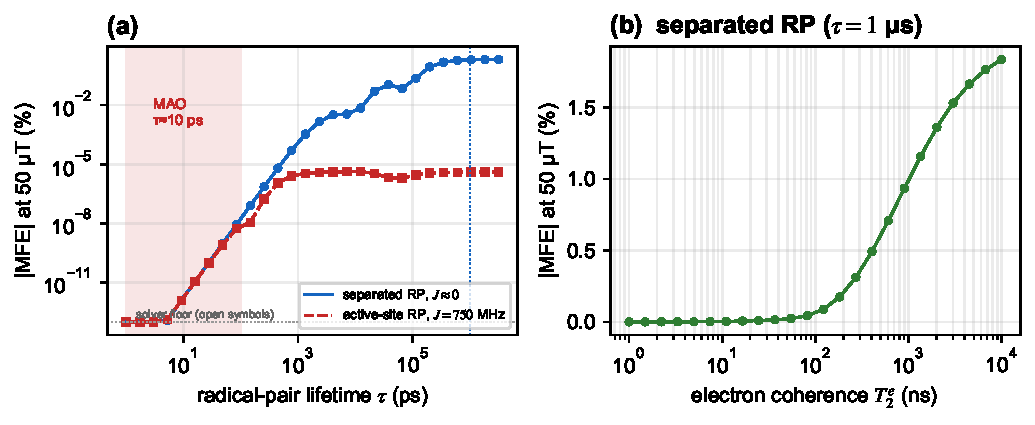
\includegraphics[width=0.92\textwidth]{fig_honest_mfe.pdf}
\caption{\textbf{Calculated geomagnetic-field sensitivity as a function of
radical-pair kinetics and electronic coherence.} All curves are computed from the
Liouville-space master equation of Eq.~\eqref{eq:me} at $B = 50\,\mu$T.
\textbf{(a)} Magnitude of the MFE versus radical-pair lifetime $\tau$ for a
spatially separated pair ($J\approx0$, $D=-9.7$~MHz, blue circles) and an
active-site pair ($J = 750$~MHz, $D=-1214$~MHz, red squares), both in the
coherent limit ($T_2^e\to\infty$). Each geometry carries its own point-dipole
coupling; $J$ and $D$ are both functions of $r$ and are not varied
independently. The separated pair requires $\tau\gtrsim40$~ns for an appreciable
effect; the active-site pair saturates at $|\mathrm{MFE}|\sim4.0\times10^{-6}\,\%$
at long lifetime. The shaded band marks the flavoenzyme regime
($\tau\approx10$~ps), where \emph{both} geometries give
$\sim\!1.7\times10^{-12}\,\%$---the lifetime, not the exchange coupling, is what
suppresses the response. Points below the solver floor (dotted line) are drawn as
open symbols; the same clamp is applied to both series. \textbf{(b)}
Magnitude of the MFE versus electronic coherence time $T_2^e$ for the optimal
separated pair ($\tau = 1\,\mu$s, $J\approx0$): a weak-field effect survives only
when $T_2^e\gtrsim180$~ns. The active-site value $T_2^e\sim1$~ns lies far below
this threshold.}
\label{fig:honest}
\end{figure*}

\begin{figure*}
\centering
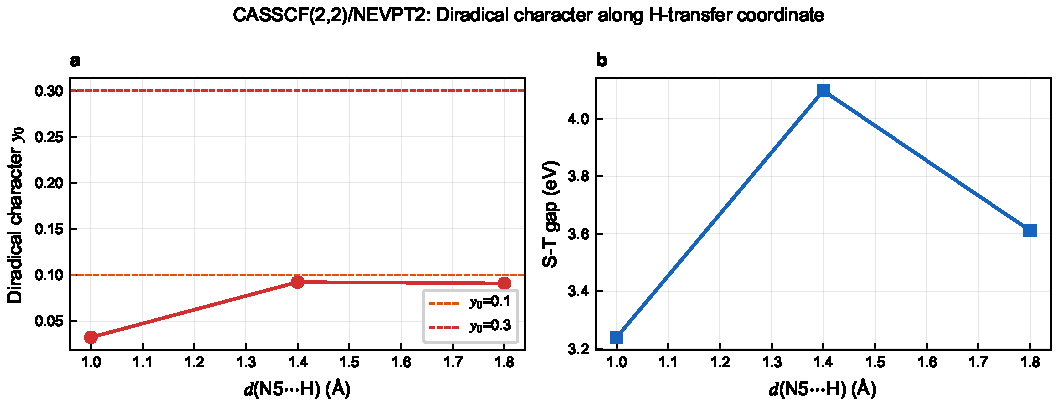
\includegraphics[width=0.78\textwidth]{fig_casscf_diradical.pdf}
\caption{\textbf{Calculated diradical character of the MAO transition state.}
CASSCF(2,2)/NEVPT2 results on a lumiflavin--methylamine model along the
hydrogen-transfer coordinate $d(\mathrm{N5}\cdots\mathrm{H})$. \textbf{(a)}
Diradical character index $y_0$ stays at $0.03$--$0.09$, well below the
$y_0 = 0.3$ guide line, indicating weak open-shell character. \textbf{(b)} The
singlet--triplet gap remains $3.2$--$4.1$~eV throughout. Both quantities are
inconsistent with formation of a low-lying, spin-correlated radical pair,
favouring a polar/concerted mechanism.}
\label{fig:casscf}
\end{figure*}

\section*{Author contributions}
Conceptualization, H.W.; methodology, H.W.; software, H.W.; validation, H.W. and
T.T.; formal analysis, H.W.; writing---original draft preparation, H.W. All
authors have read and agreed to the published version of the manuscript.

\section*{Conflicts of interest}
There are no conflicts to declare.

\section*{Data availability}
The source code, parameter files, and analysis scripts supporting this article are
openly available in the \texttt{qbscreen} Python package at
\url{https://github.com/deeptell-inc/brain_protein_screening} under the MIT
licence. This includes the Liouville-space master-equation solver, the per-enzyme
magnetic-field-effect driver, and an automated test suite. The suite pins the
values of Table~1 to within 2\% by direct recomputation, checks the solver against
a closed-form coherent-limit expression, and verifies the $B^2$ scaling of the
computed MFE reported in the ESI\dag\ (Table~S1). We note that the closed-form
check shares the eigenbasis convention of the solver and therefore validates the
Liouville-space inversion rather than the unit conventions; the $B^2$ test does
not, and is in that sense the independent one. A versioned snapshot
will be archived on Zenodo with a citable DOI upon acceptance.

\section*{Acknowledgements}


%%%END OF MAIN TEXT%%%

%The \balance command can be used to balance the columns on the final page if desired. It should be placed anywhere within the first column of the last page.

\balance

%If notes are included in your references you can change the title from 'References' to 'Notes and references' using the following command:
%\renewcommand\refname{Notes and references}

%%%REFERENCES%%%
\bibliography{refs} %You need to replace "rsc" on this line with the name of your .bib file
\bibliographystyle{rsc} %the RSC's .bst file
\end{document}
